\chapter{نمودار بسته تحلیل}

در ادامه نمودار بسته‌های تحلیل برای کلاس‌های گفته شده در فصل
\ref{chapter:classAnalysis}
آورده شده است. در قسمت ارتباطات بسته‌ها با یکدیرگ، به دلیل جلوگیری از پیچیدگی بیش‌از‌اندازه شکل، اجزای درونی بسته‌ها رسم نشده است.


\begin{figure}[ht!]
	\centering
	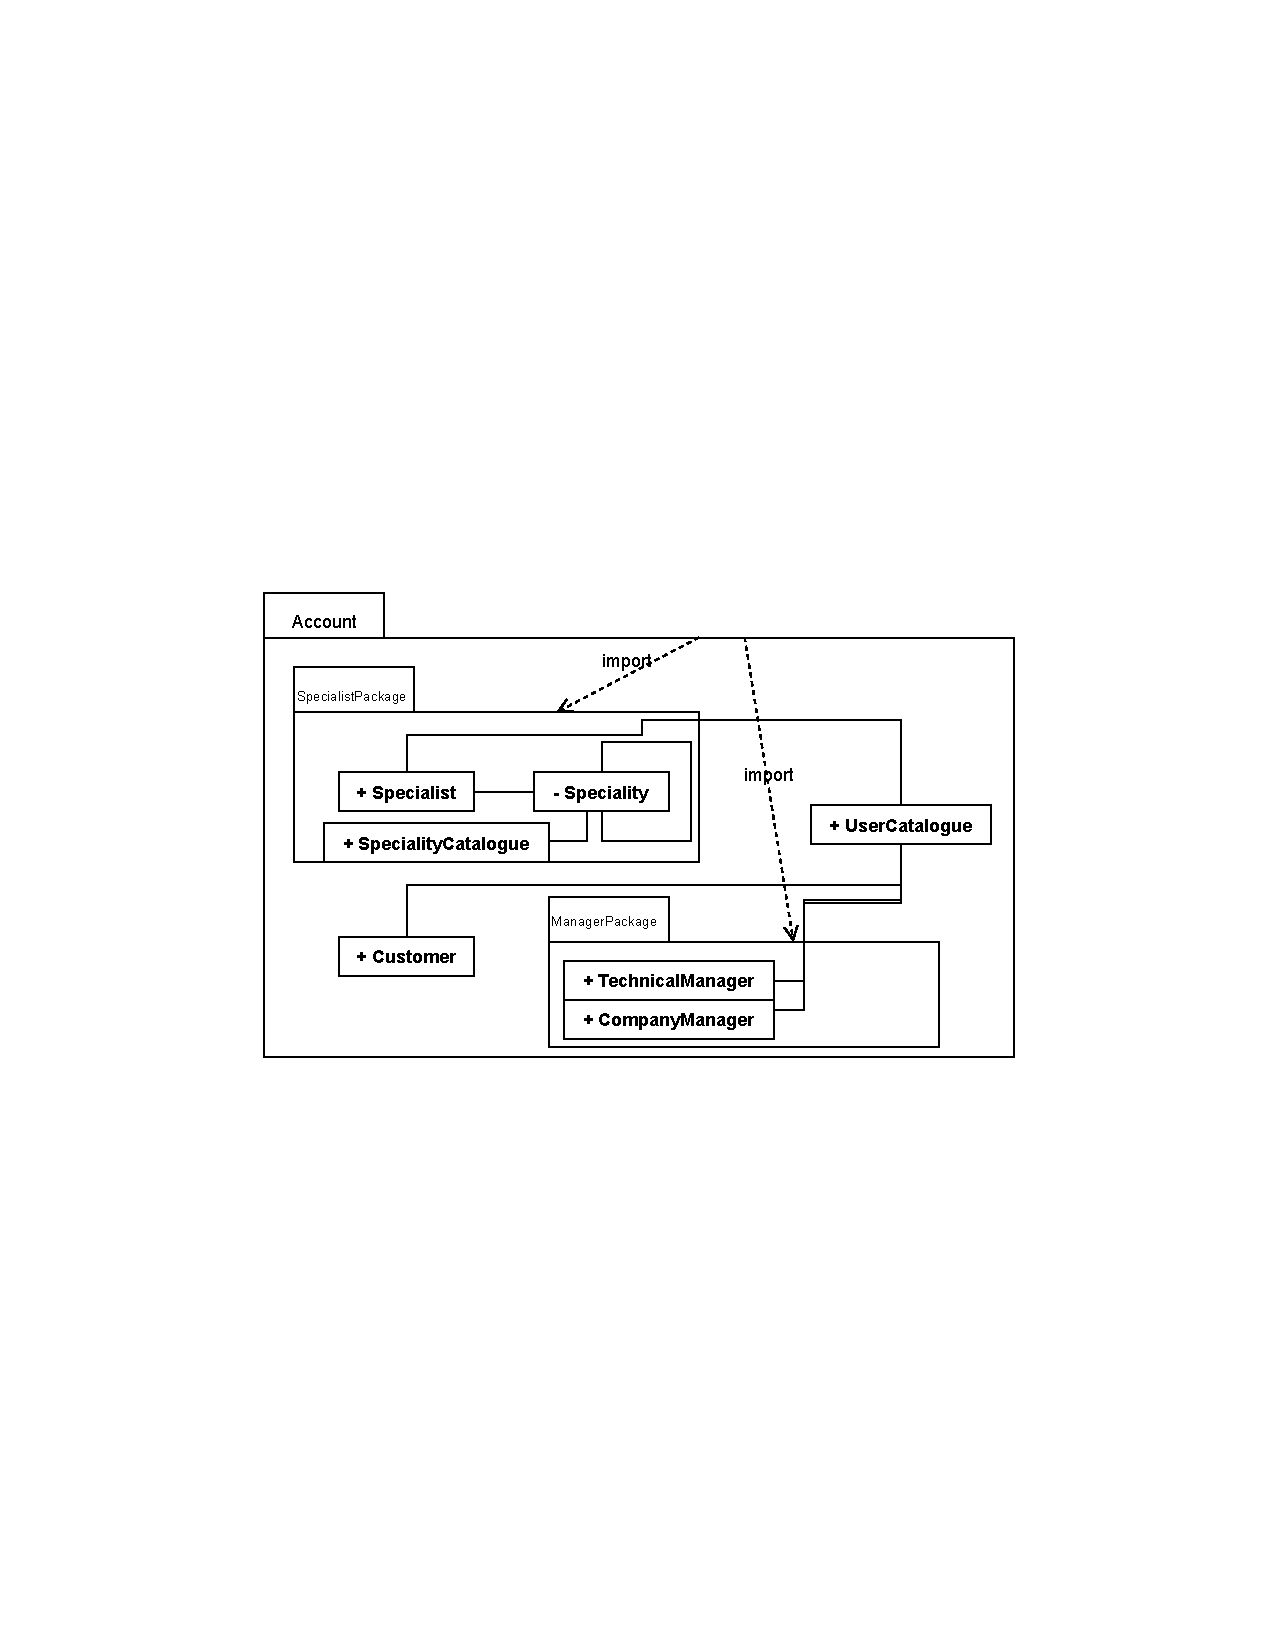
\includegraphics[scale=0.8]{figs/OOD-package-1.pdf}
	\caption{نمودار بسته: بسته \lr{Account}}
\end{figure}
\FloatBarrier
\newpage

\begin{figure}[ht!]
	\centering
	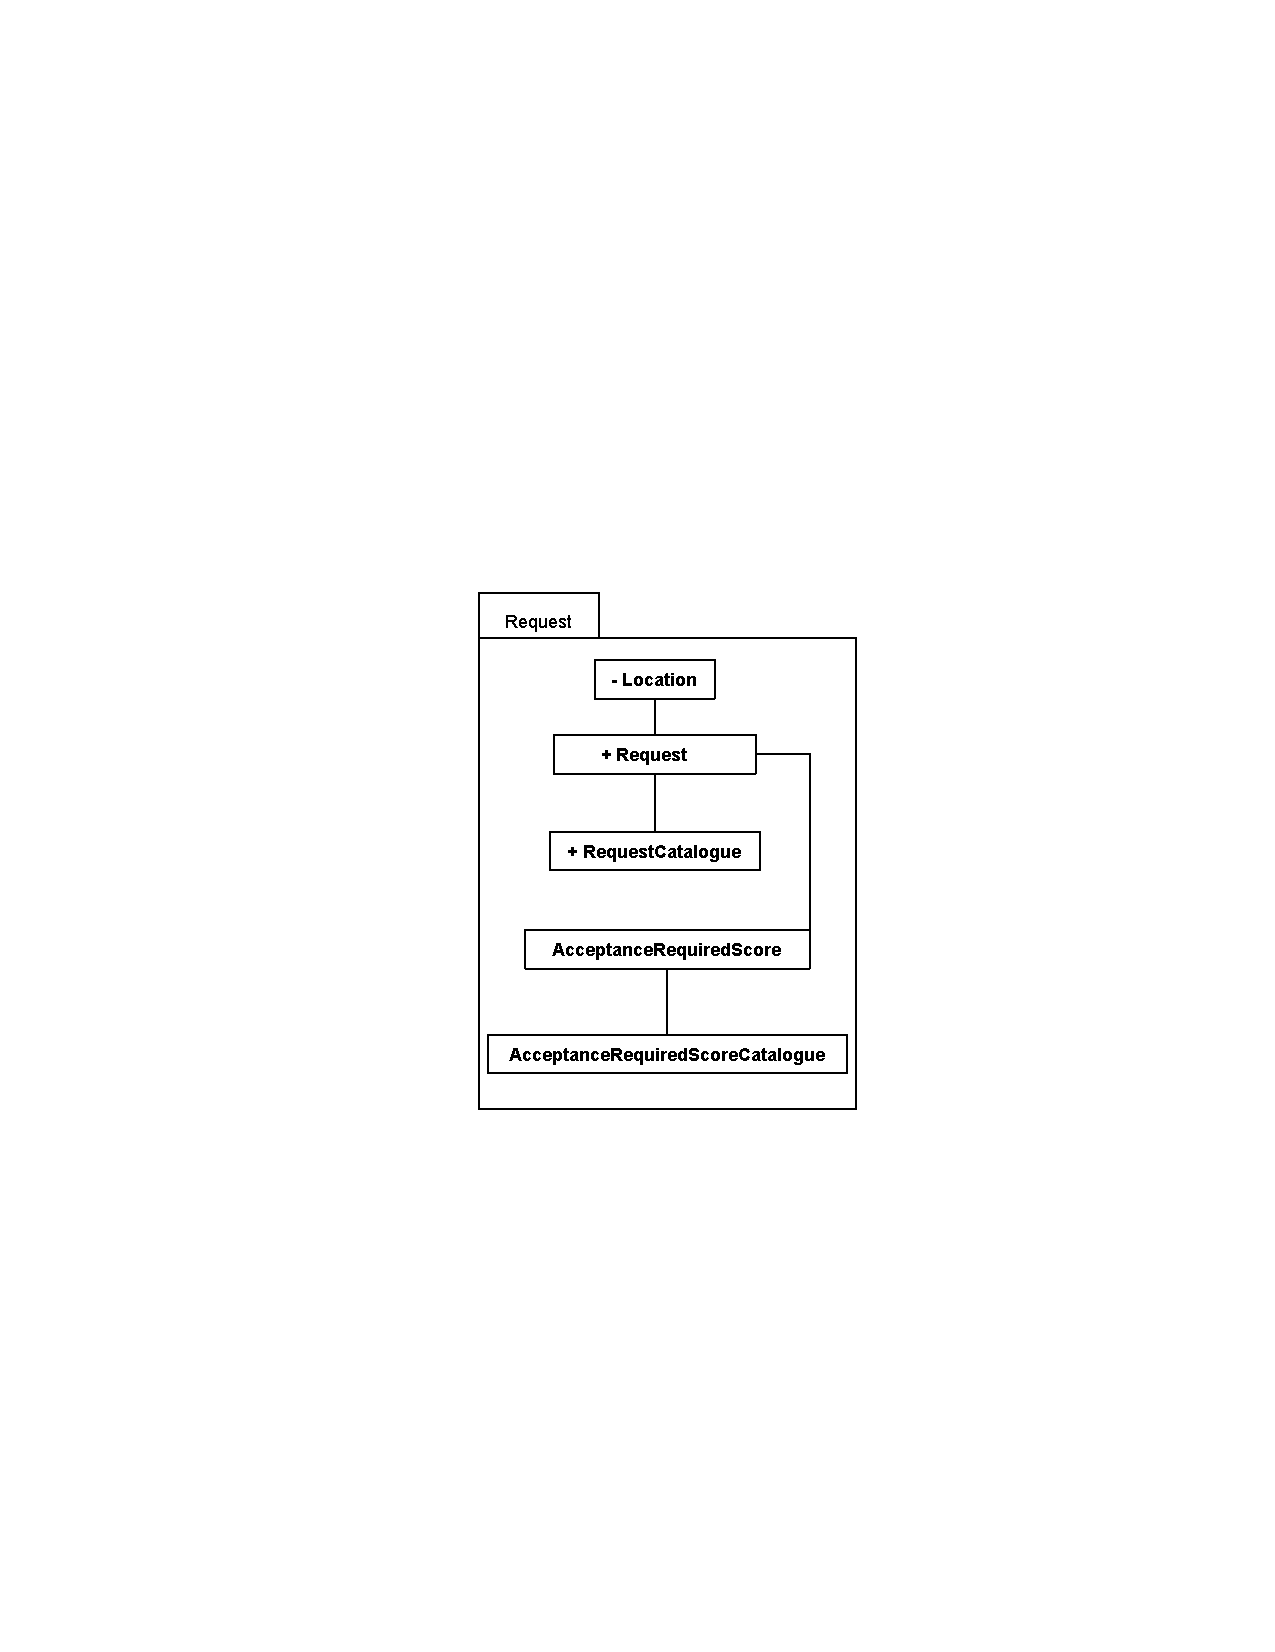
\includegraphics[scale=0.8]{figs/OOD-package-2.pdf}
	\caption{نمودار بسته: بسته \lr{Request}}
\end{figure}
\FloatBarrier
\newpage


\begin{figure}[ht!]
	\centering
	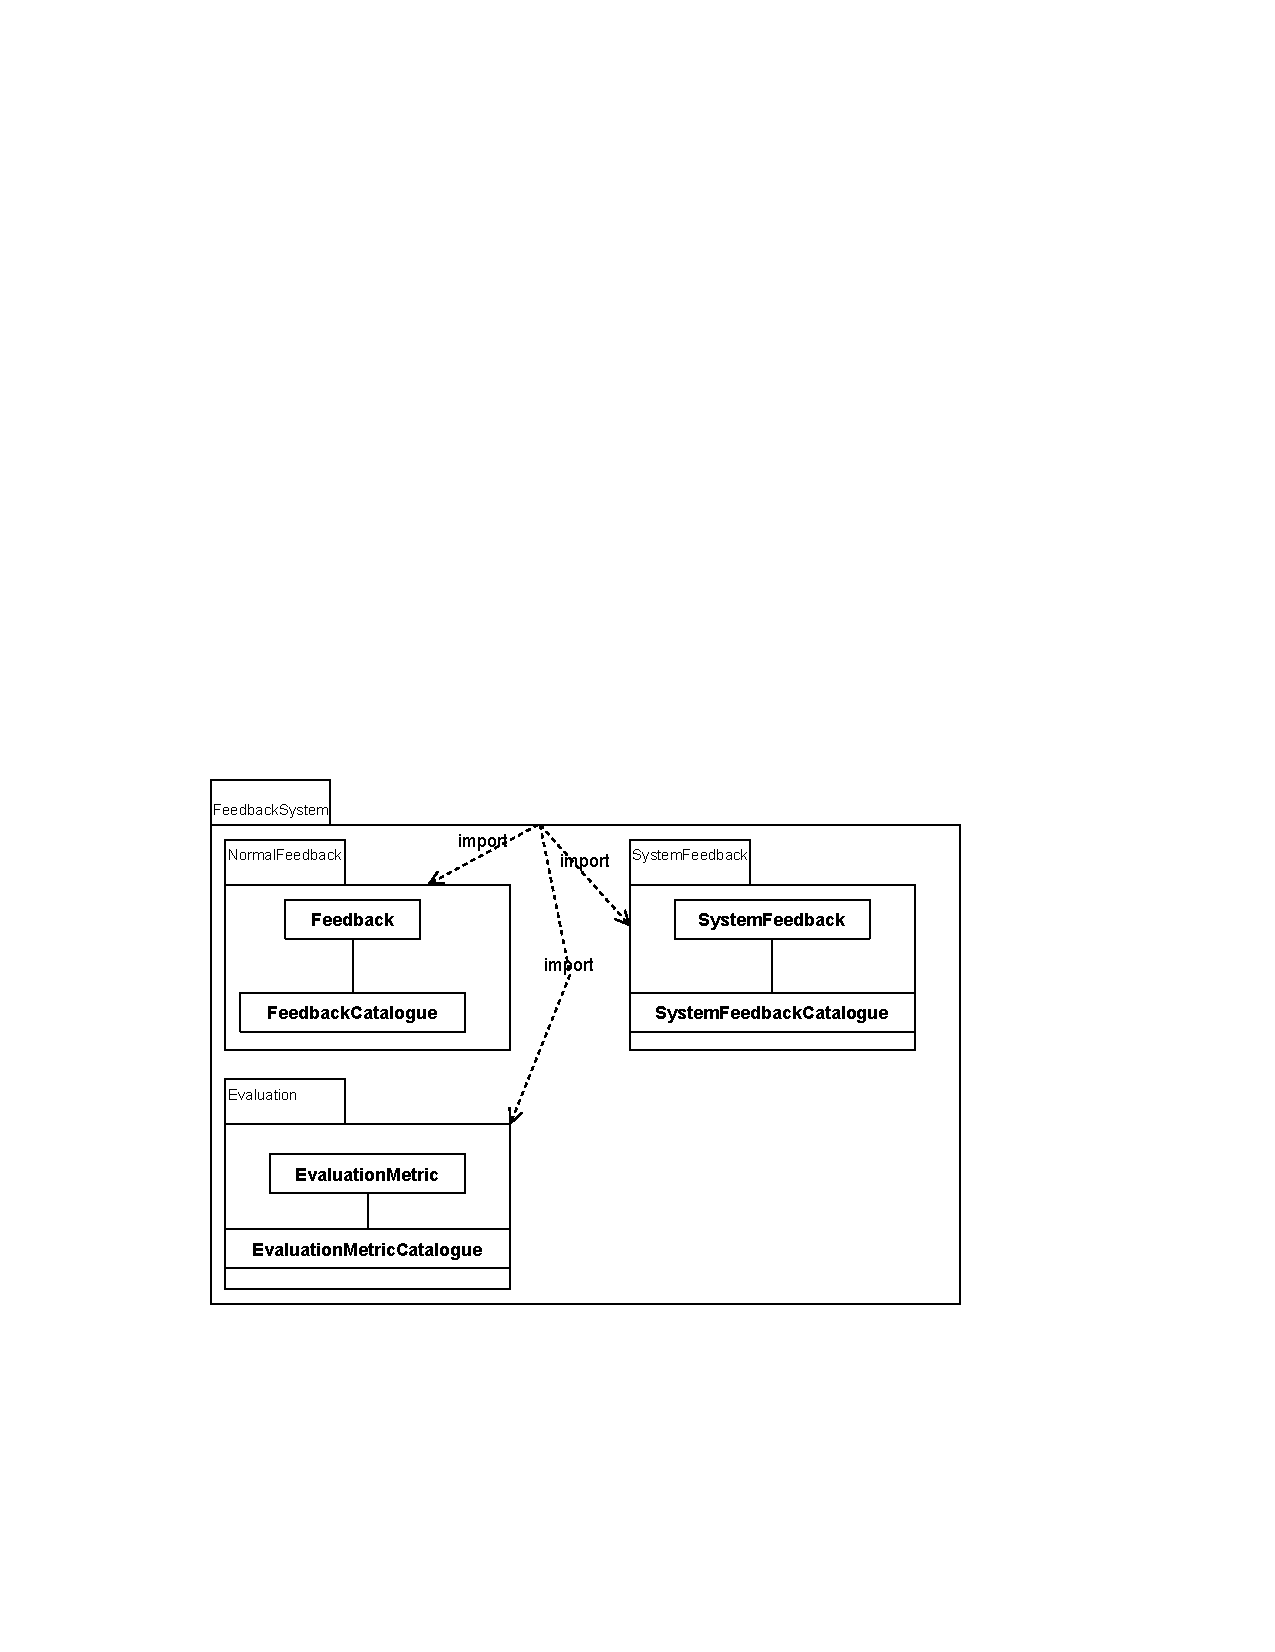
\includegraphics[scale=0.8]{figs/OOD-package-3.pdf}
	\caption{نمودار بسته: بسته \lr{FeedbackSystem}}
\end{figure}
\FloatBarrier
\newpage

\begin{figure}[ht!]
	\centering
	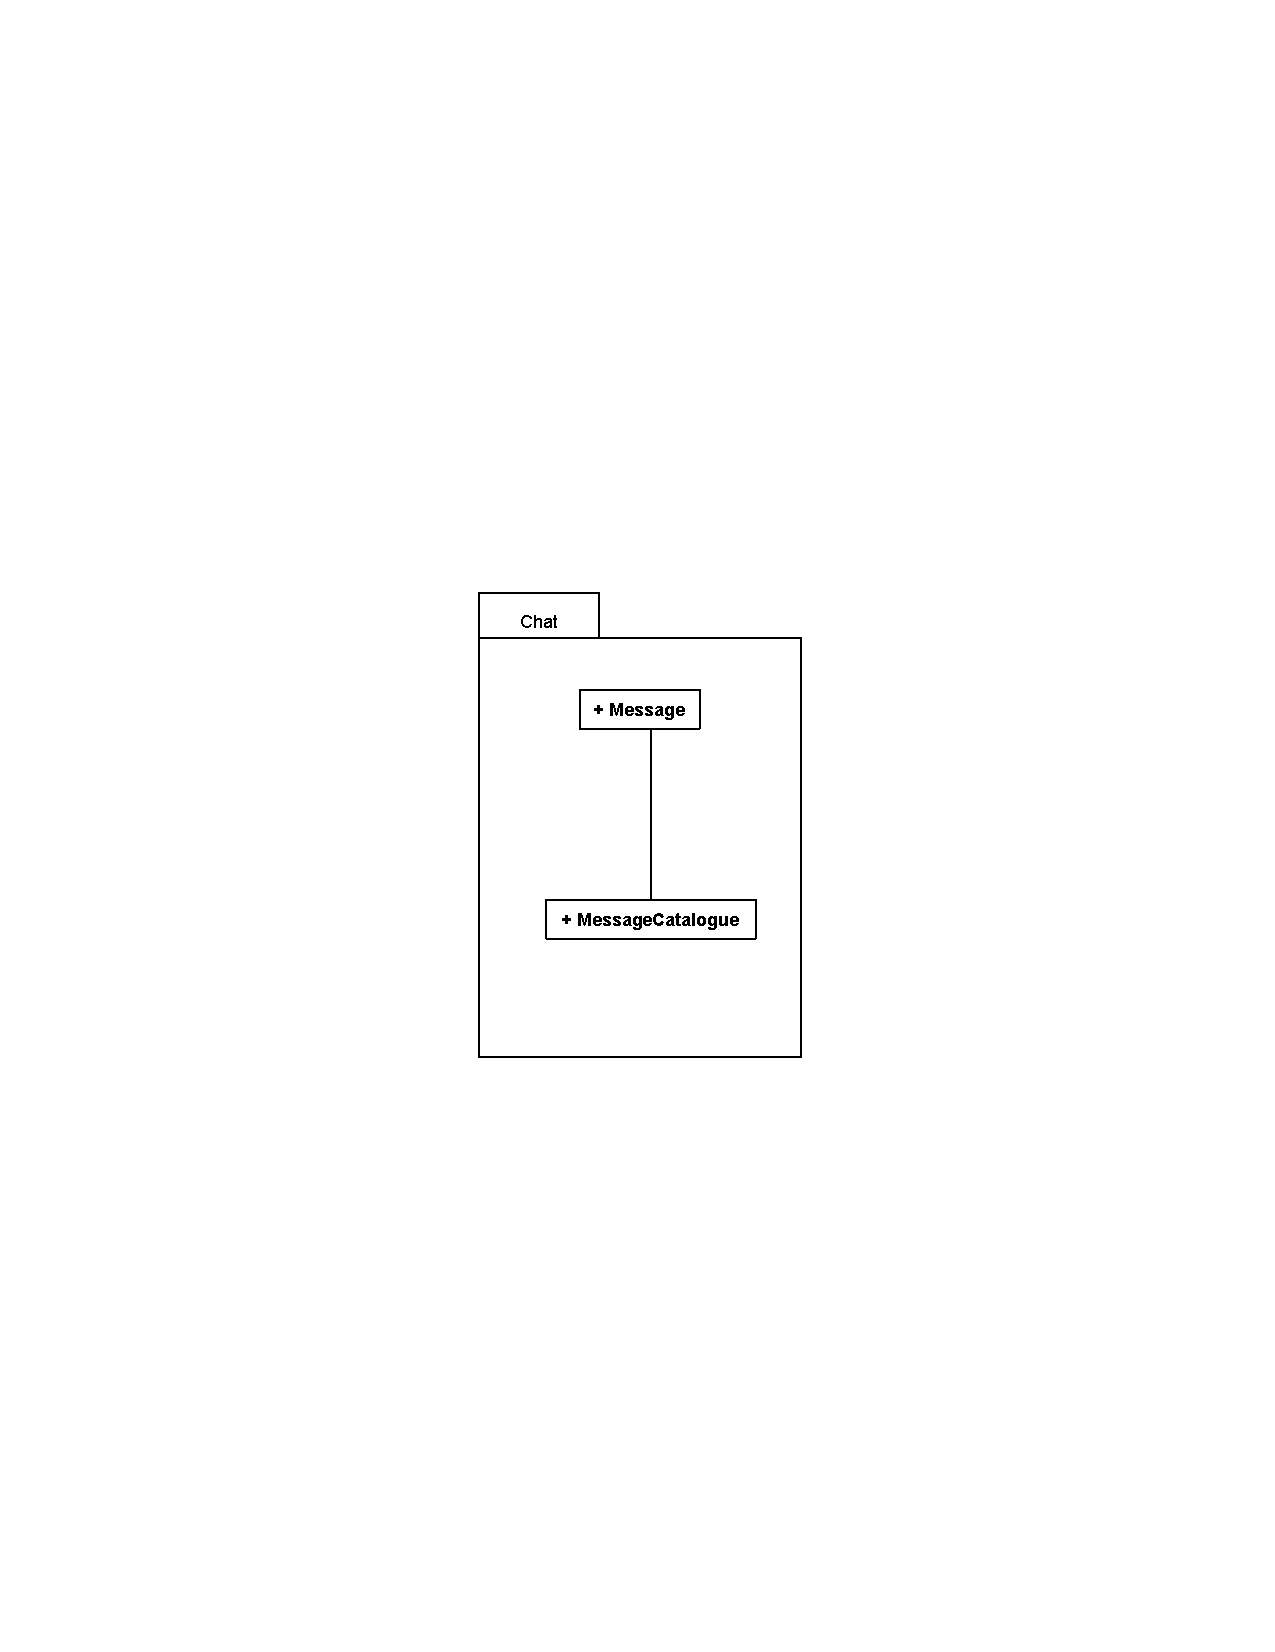
\includegraphics[scale=0.8]{figs/OOD-package-4.pdf}
	\caption{نمودار بسته: بسته \lr{Chat}}
\end{figure}
\FloatBarrier
\newpage

\begin{figure}[ht!]
	\centering
	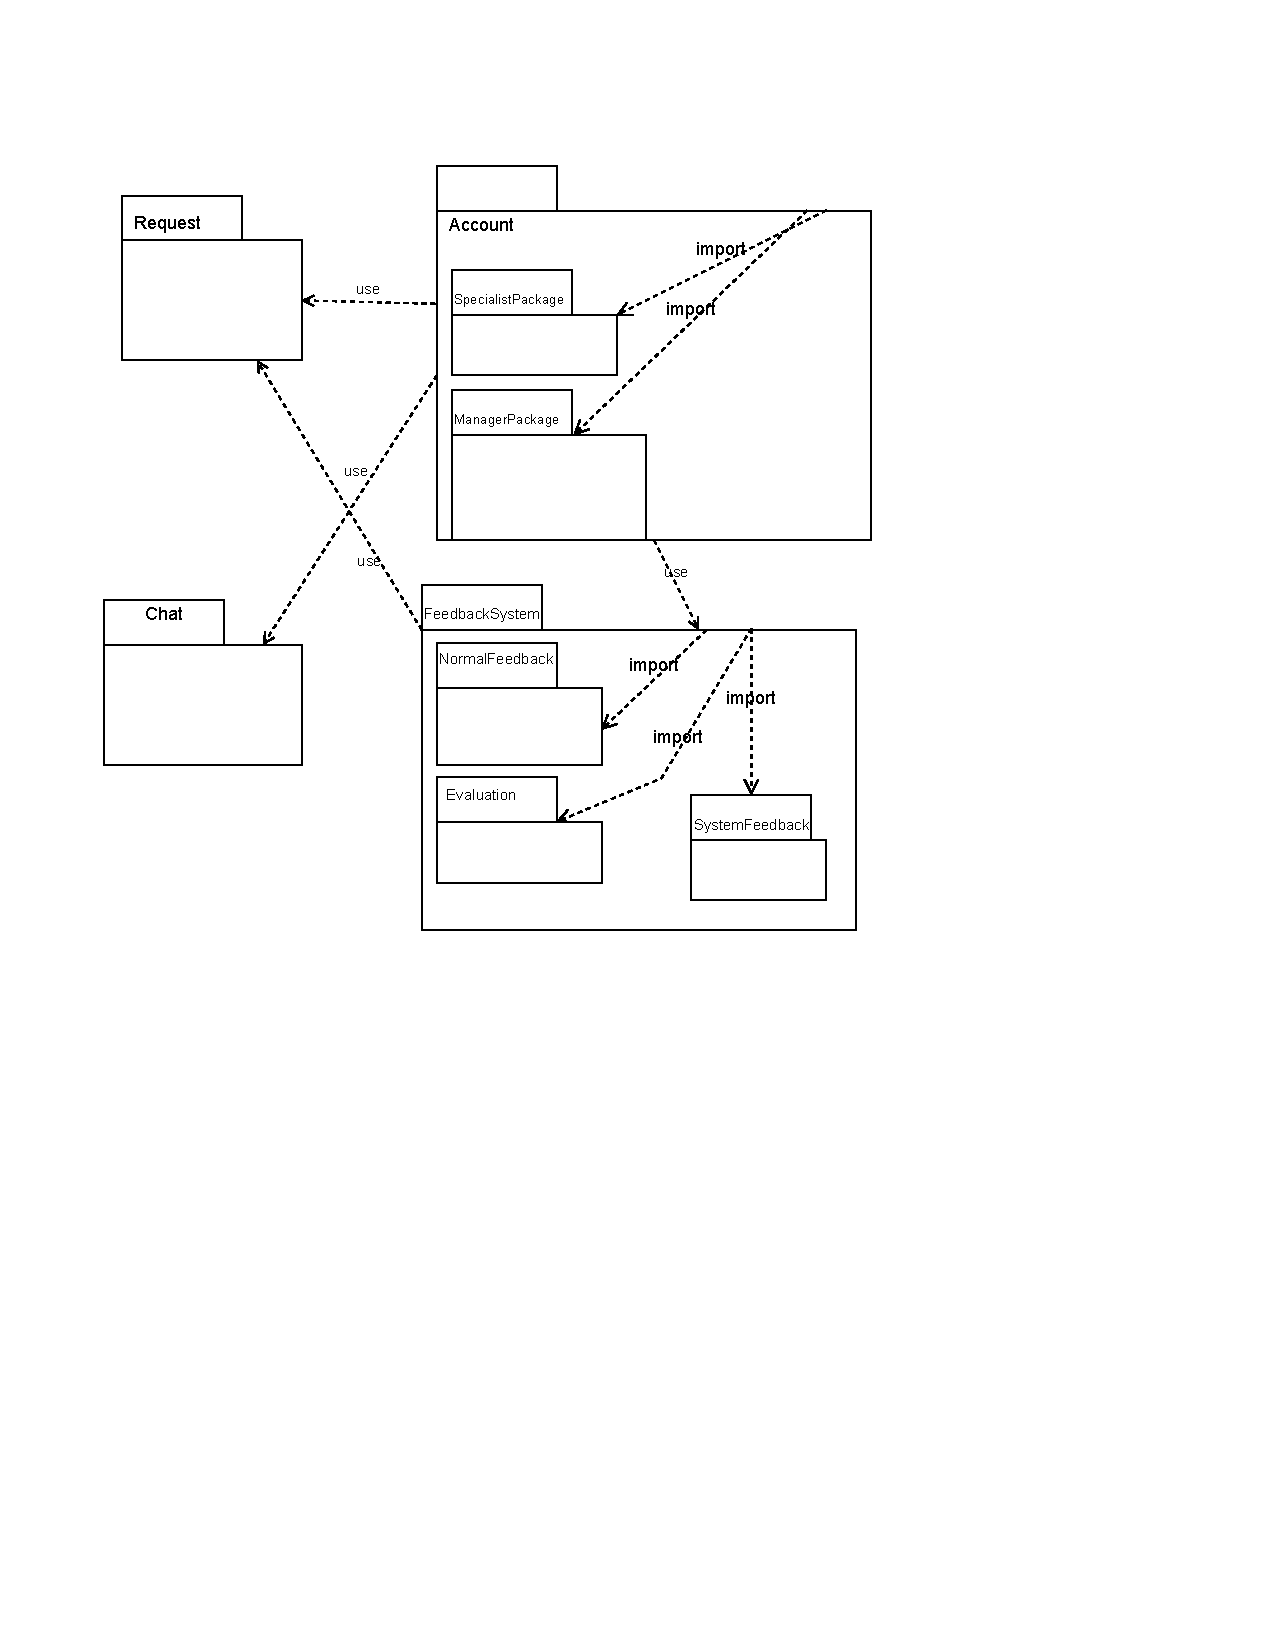
\includegraphics[scale=0.8]{figs/OOD-package-5.pdf}
	\caption{نمودار بسته:  ارتباط بسته‌ها با یکدیگر}
\end{figure}
\FloatBarrier
\newpage

